\part{Introduction}
\lecture{Introduction}{Introduction}
\section{Introduction}

\title{Ordinary Differential Equations}
\subtitle{Introduction}
\date{26 Aug 2013}

\begin{frame}
  \titlepage
\end{frame}

\begin{frame}
  \frametitle{Outline}
  \tableofcontents[hideothersubsections,sectionstyle=show/hide]
\end{frame}

\subsection{Syllabus}
\begin{frame}
  \frametitle{Syllabus}

  Read the syllabus! The syllabus will take precedence over any
  discrepancies here. It includes \textbf{all} of our policies. We
  will not cover them all here.

  Faculty: \\
  \begin{tabular}{l@{\hspace{3em}}l@{\hspace{3em}}l}
    Kelly Black                      & Guangming Yao    \\
    361B Science Center              & 363 Science Center   \\
    268-3831                         & 268- 6496\\
    kjblack@gmail.com                &  gyao@clarkson.edu\\ [10pt]
  \end{tabular}

\end{frame}


\begin{frame}
  \frametitle{Materials}

  \begin{itemize}
  \item {\em Differential Equations and Linear Algebra}, second
    edition
  \item Recitation manual \\
    The UPS Store, \\
    200 Market St, \\
    315.265.4565, \\
    store5986$@$theupsstore.com
  \item Turning Point Technologies ResponseCard RF LCD clicker \\
    \url{https://store.turningtechnologies.com} \\
    The Clarkson University promotional code is Z0k0.
  \end{itemize}
  
\end{frame}


\begin{frame}
  \frametitle{Test Dates}

  The tests will be given 24 September, 29 October,
  and 19 November. The exams will take place in the evenings from
  7:00pm to 8:20pm. You should bring your own pencils.  The professor
  will not have any spare materials. The location will vary depending
  on your recitation section, and your room assignments will be given
  prior to the exams.
  
\end{frame}


\begin{frame}
  \frametitle{Grading}

   \begin{tabular}[t]{rl}
    40\% & 3 Tests. \\
    15\% & Final Exam. \\
    15\% & Homework and Webwork. \\
    15\% & Quiz. \\
    10\% & Projects\\
     5\% & Clickers
  \end{tabular}

  \begin{itemize}
  \item The right to miss a scheduled exam and take a make up exam can
    be awarded only by your professor.
  \item If for some reason you must miss an exam, you must apply in
    writing {\bf before} the exam.
  \item In case of emergency contact the professor as soon as possible
    and provide documentation to confirm why you cannot take part in
    the exam. 
  \item An unexcused absence will result in a grade of zero on the
    exam.
  \end{itemize}


  
\end{frame}


\begin{frame}
  \frametitle{Academic Accommodations}

  If you require any kind of special
  accommodation please see your professor.  Requests for academic
  accommodations must be made during the first three weeks of the
  semester, except for unusual circumstances.  Students must register
  with the Office of Accommodative Services, located in the Student
  Success Center, 110 ERC, to verify their eligibility for appropriate
  accommodations.
  
\end{frame}

\begin{frame}
  \frametitle{Clickers}

  We will start using the clickers this Friday. Each day one or more
  questions will be asked.

  You need to register your clicker. Go to our course page on moodle:
  \begin{enumerate}
  \item Choose the ``clicker ID'' option at the top of the page.
  \item Enter your clicker Device ID (found on the back of the
    clicker.)
  \item Click on the submit button.
  \item Click on the ``next'' button.
  \item Click on ``Submit all and finish.''
  \item Confirm your choice.
  \item Click on ``Finish Review'' at the bottom of the page.
  \end{enumerate}

  If you do not click on ``Finish Review'' your device ID may not be saved.
   
  
\end{frame}


\begin{frame}
  \frametitle{Projects}
\begin{itemize}
\item Projects There will be two projects. 
\item The first project will be given on 11 September and will be
due on 19 September. 
\item The second project will be given on 6 November and will be due on 14
November.
\end{itemize}
\end{frame}



\begin{frame}
  \frametitle{Recitations}

  \begin{itemize}
  \item Take place every Thursday.
  \item Will have a quiz almost every session.
  \item Some days the quiz will consist of the pre-class activity in
    your lab manual. (Random!)
  \item The recitation is where you \textbf{DO} things. It is where
    you will learn the most in this class.
  \end{itemize}
\end{frame}

\begin{frame}{Expectations}\small
  Our evaluation is based on the following expectations: \\
  \hspace*{-2em}
\begin{tabular}{|l@{\hspace{2em}}l|} \hline
  Quality of Work    & Expectations \\ \hline
  Needs Improvement  & Cannot identify basic equations \\
                     & Cannot determine solutions for basic \\
                     & systems of equations \\ \hline
  Satisfactory       & Can identify and solve all basic equations \\ 
                     & Can determine stability characteristics of \\
                     & all basic equations \\ \hline
  Good               & Derive own systems \\
                     & Determine solutions and stability of own systems \\ \hline
  Excellent          & Tie together linear algebra concepts to \\
                     & solution techniques \\
                     & Can determine solution to any one system using \\
                     & a variety of techniques \\ \hline
\end{tabular}
\end{frame}

\subsection{What is a Differential Equation}

\begin{frame}{Topics}\small
\begin{tabular}{|l@{\hspace{2em}}l|} \hline
  Topic & Important Ideas \\  \hline
  First Degree Equations  & Linear Equations, Nonlinear Equations, \\
                          & Laplace Transforms \\ \hline
  Second Degree Equations & Linear Equations, Cauchy-Euler Equations, \\
                          & Laplace Transforms \\ \hline
  Systems of Equations    & Linear Algebra, Eigen Systems \\ \hline
  Modeling and Stability  & Mathematical Models, Qualitative Behavior \\ \hline
\end{tabular}

\centerline{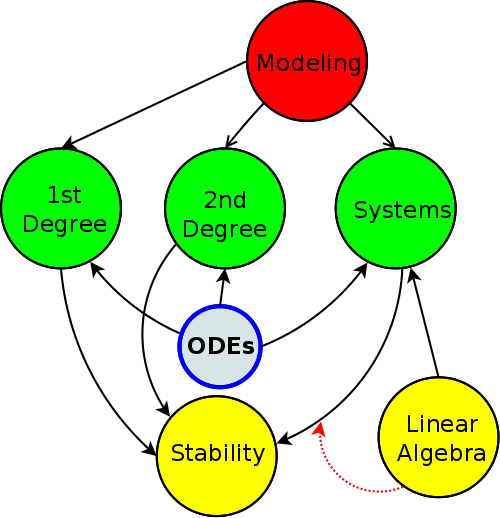
\includegraphics[height=12em]{img/topics}}
\end{frame}


\begin{frame}
  \frametitle{What is a DE?}

  Given
  \begin{eqnarray*}
    y'(x) & = & y(x),
  \end{eqnarray*}
  what is $y(x)=?$

  \begin{eqnarray*}
    \deriv{y(x)}{x} & = & y(x)
  \end{eqnarray*}

\end{frame}


\begin{frame}{Question:}
  Given
  \begin{eqnarray*}
    y'' + 3y' +2y & = & 0
  \end{eqnarray*}

  what is $y(x)$?

  \uncover<2->{
    Note: we leave often leave off the function notation.
    }

  \uncover<3->{
    Why? We are lazy!
    }

\end{frame}

\begin{frame}
  \frametitle{Notation}
  \begin{eqnarray*}
    \dot{y} & = & \deriv{y}{t} \\
    \only<2->{\ddot{y} & = & \derivTwo{y}{t} }\\
    \only<3->{y' & = & \mathrm{depends.... usually ~~} \deriv{y(x)}{x} }\\
    \only<4->{y'' & = & \derivTwo{y(x)}{x} }
  \end{eqnarray*}
\end{frame}

\begin{frame}
  \frametitle{Nomenclature}
  
  \vfill

  $\deriv{y}{x}$ - then ``ordinary differential equation.''

  \vfill

  $\frac{\partial y}{\partial x}$ - then ``partial differential
  equation.''

  \vfill

  Order is the highest number of derivatives:
  \begin{eqnarray*}
    y'' - 3 y' + 2y & = & 0, \mathrm{second~order} \\
    y'  & = & 4y, \mathrm{first~order} 
  \end{eqnarray*}

  \vfill


\end{frame}

\subsection{Modeling}


\begin{frame}
  \frametitle{Modeling}

  Why bother?

  Many ``mathematical models'' provide a relationship between rates.

  ex: Newton's Second Law, ``$\vec{F} = m \vec{a}$'' In 1 dimension:
  \begin{eqnarray*}
    m\mathrm{~(acceleration)} & = & \sum_i \lp F \rp_i, \\
    m \ddot{x} & = & \sum_i \lp F \rp_i
  \end{eqnarray*}

  
\end{frame}


\begin{frame}
  \frametitle{Circuit}
  
  The voltage across a resistor is proportional to the current flowing
  through it.

  \only<2->
  {
    There is some number, R, where
    \begin{eqnarray*}
      V & = & IR
    \end{eqnarray*}
  }
\end{frame}

\begin{frame}
  \frametitle{Proportionality}
  
  If $a$ is proportional to $b$ then there is a constant, $k$, where 
  \begin{eqnarray*}
    a  & = & k \cdot b
  \end{eqnarray*}

  if $a$ is inversely proportional to $b$ then there is a constant $c$
  where 
  \begin{eqnarray*}
    a & = & c \frac{1}{b}
  \end{eqnarray*}
\end{frame}

\begin{frame}
  \frametitle{Example - Newton's Law of Cooling}

  The rate of change of the temperature of an object is proportional
  to the difference between the object and its surroundings (the
  ambient temperature).

  \uncover<2->
  {

    Define:
    \begin{itemize}
    \item $T(t)$ is the temperature at a time $t$.
    \item $A$ is the ambient temperature (the temperature of the
      surroundings).
    \item The rate of change of the temperature is $\frac{dT(t)}{dt}$.
    \end{itemize}

  }

  \uncover<3->
  {

    There is some constant number, $k$, where 
    \begin{eqnarray*}
      \frac{dT(t)}{dt} & = & -k (T-A).
    \end{eqnarray*}

  }


\end{frame}


\begin{frame}
  \frametitle{Newton's Law of Cooling}

  The rate of change of the temperature of an object is proportional
  to the difference between the object and its surroundings (the
  ambient temperature).

    There is some constant number, $k$, where 
    \begin{eqnarray*}
      \frac{dT(t)}{dt} & = & -k (T-A).
    \end{eqnarray*}

    Question: What is the temperature at any given time?

\end{frame}


\begin{frame}{Extra Topic (Outside of class) }

  Checking your solution:
  \begin{itemize}
  \item You have a differential equation.
  \item You have a function that you think is the solution.
  \end{itemize}

  How do you check to see if it is correct?

  \uncover<2>{\color{red} You plug it back into the equation!}

  \uncover<3>{This is something that causes a large amount of
    confusion. If you are asked to \textbf{check} a solution you only
    need to plug it back into the equation and see if the
    \blueText{left side} is equal to the \fuchsiaText{right side} of
    the equation. This also means that you can always check your work
    using the skills you learned in Calculus I.}
  
\end{frame}


\begin{frame}{Example}

  Show that {\color{red} $y=t\cos(t)$} is a solution to the differential equation
  \begin{eqnarray*}
    \blueText{y' - \frac{1}{t}y} & = & \fuchsiaText{-t\sin(t)}.
  \end{eqnarray*}

  \only<2>{

    \begin{itemize}
    \item We will take the necessary derivatives of the function. (In this
      case one.)
    \item We will plug it into the equation.
    \item We will check to see if the \blueText{left hand side} is
      equal to the \fuchsiaText{right hand side}.
    \end{itemize}

  }

  \only<3-5>{

    \begin{eqnarray*}
      \redText{y} & = & \redText{t\cos(t)}, \\
      y' & = & \cos(t) - t\sin(t).
    \end{eqnarray*}
  }

  \only<4->{

    Plug the result into the left hand side of the equation:
    \begin{eqnarray*}
      \blueText{y' - \frac{1}{t}y} & = & \cos(t) - t\sin(t) - \frac{1}{t} t \cos(t), \\
      & = & \cos(t) - t\sin(t) - \cos(t), \\
      & = & -t\sin(t).
    \end{eqnarray*}

  }

  \only<5->{

    Plug the result into the right hand side of the equation (easy in
    this case!):
    \begin{eqnarray*}
      \fuchsiaText{-t\sin(t)}.
    \end{eqnarray*}

  }

  \only<6->{

    Note the result.... They are the same! The function satisfies the
    differential equation so it is \textbf{a} solution. Note that if
    there had been extra conditions we would have to check
    \textbf{all} of them.

  }
  
\end{frame}


% LocalWords:  Clarkson pausesection hideothersubsections sectionstyle Yao
% LocalWords:  Guangming ResponseCard Webwork moodle
